\section{Система мониторинга Zabbix}

Для решения проблемы недостаточного контроля ресурсов сетевого и серверного оборудования был выбран и использован Zabbix.

Основные критерии при выборе были:
\begin{itemize}
\item свободная лицензия;
\item поддержка SNMP;
\item гибкая система шаблонов и групп;
\item автоматическое обнаружение.
\end{itemize}

В нашем проекте Zabbix был использован для:
\begin{itemize}
\item мониторинга состояния сети;
\item контролирование ресурсов сервера;
\end{itemize}

Была проделана следующая работа:
\begin{itemize}
\item был обновлен и настроен Zabbix-сервер;
\item для игрового оборудования были написаны шаблоны для получения данных по SNMP и проверка на доступность;
\item для сервера был установлен и настроен Zabbix-агент;
\item было автоматизирован поиск и добавление zabbix-агентов в систему.
\end{itemize}

В самом начале был написан шаблон получения данных с маршрутизаторов. Вот так выглядят получаемые данные (рисунок \ref{img:9}).

\begin{figure}[h!]
    \centering
    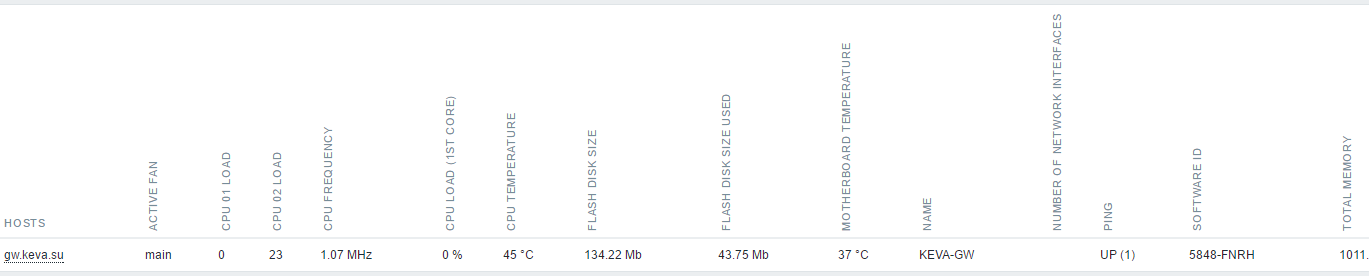
\includegraphics[width=1\textwidth]{9}
    \caption{Получаемые данные с оборудования}
    \label{img:9}
\end{figure} 

Для автоматизации процесса было решено сделать проверку на доступность и триггер на срабатывание (рисунок \ref{img:10}).

\begin{figure}[h!]
    \centering
    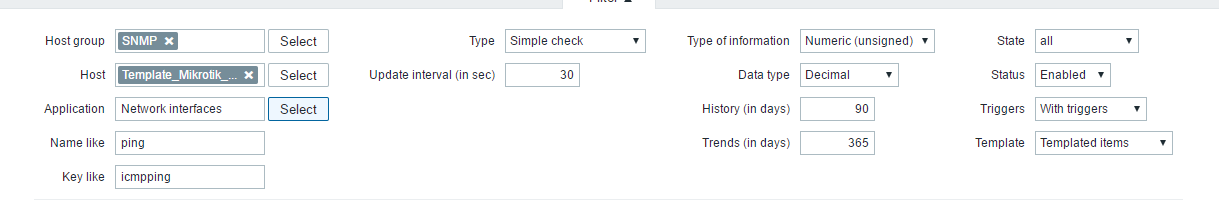
\includegraphics[width=1\textwidth]{10}
    \caption{Проверка на доступность}
    \label{img:10}
\end{figure} 

Также был настроен автоматизированный поиск агентов в указанной сети. Во время игры агенты будут предустановлены на виртуальные машины и при запуске игры система сама добавит их в свой список мониторинга (рисунок \ref{img:11}).

\begin{figure}[h!]
    \centering
    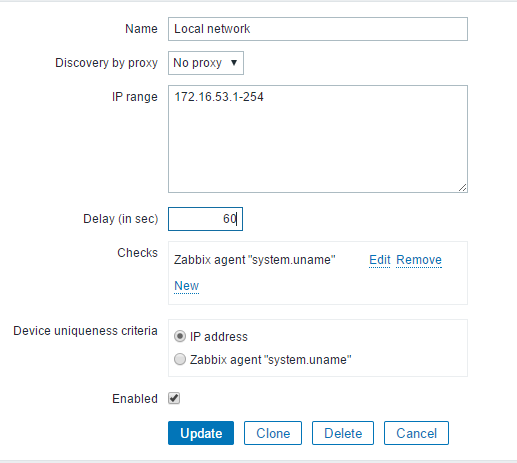
\includegraphics[width=0.8\textwidth]{11}
    \caption{Правило автоматического обнаружения}
    \label{img:11}
\end{figure} 

После данных настроек Zabbix-сервер готов для использования на SibirCTF в автоматизированном режиме.\\